\subsection{Will I get the dukedom promised by the King?}
\begin{frame}[t]{Will I get the dukedom promised by the King?}
\begin{columns}[T, onlytextwidth]
\column{0.5\textwidth}
\Jupiter\ is L1, direct, in the 10th (most elevated planet) \\
\hspace{1em}\Sun\ \& \Venus\ $\Rightarrow$ \Square\ from \Sagittarius\ on 1st (received) \\
\hspace{1em}aspects both his domiciles \Sagittarius\ (1st) and \Pisces\ (4th) \\
\hspace{1em}aspects the 7th (connections to all 4 angles) \\
\hspace{1em}signifying he will get his dukedom\\
\vspace{0.5em}
\Mercury\ is L7, retro, a rebel opponent in the matter \\
\hspace{1em}cadent in the 12th \\
\hspace{1em}$\Rightarrow$ \Opposition\ \Saturn\ retro, cadent in 6th\footnotemark[1] \\
\hspace{1em}signifying his opponent's destruction \\
\vspace{0.5em}
\Mercury\ retro, by transit, $\Rightarrow$ \Sextile\ \Jupiter\ with reception indicates the rebel opponent will end by seeking "peace and accommodation" from the querent

\column{0.5\textwidth}
\begin{center}
{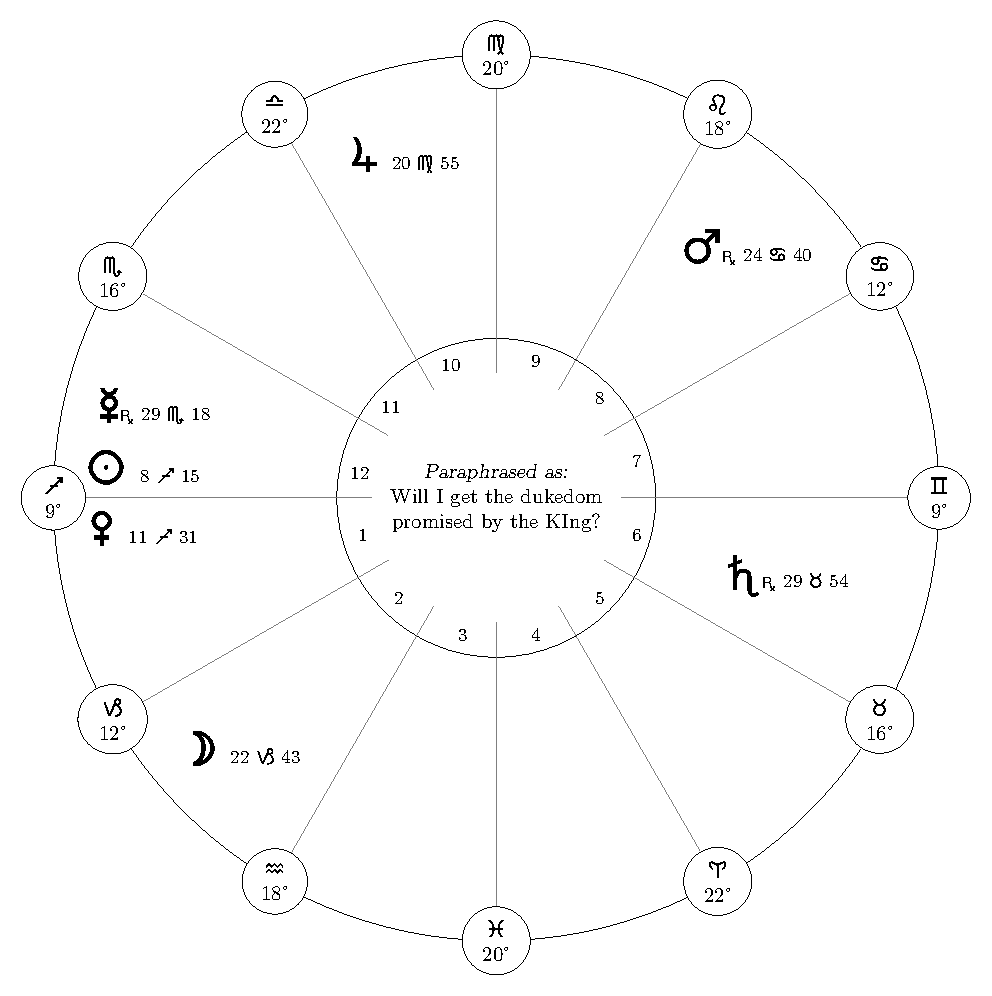
\includegraphics[width=0.9\textwidth]{charts/52-chart-dukedom}} \\
\scriptsize
The MC was not given, only the Asc degree. The other cusps are in the text Holden used but are not original to Masha'Allah.
\end{center}
\end{columns}
\footnotetext[1]{Hand notes this can only be true by Primary Direction.}

\end{frame}
% --------------------------------------------------------------
\begin{frame}[t]{Dukedom Continued}
\vspace{0.5em}
\Jupiter\ \Trine\ (not rec'd) $\Leftarrow$ \Moon\ $\Rightarrow$ \Opposition\ \Mars\ (mixed MR) \\
\hspace{1em}\Moon\ is significator of the opponent \\
\hspace{1em}\Mars\ retro, in Fall, indicating his downfall\\


\end{frame}